\documentclass{article}

% Required to support mathematical unicode
\usepackage[warnunknown, fasterrors, mathletters]{ucs}
\usepackage[utf8x]{inputenc}

% Always typeset math in display style
%\everymath{\displaystyle}

% Use a larger font size
\usepackage[fontsize=12pt]{scrextend}
\usepackage[margin=1in]{geometry}

% Standard mathematical typesetting packages
\usepackage{amsfonts, amsthm, amsmath, amssymb}
\usepackage{mathtools}  % Extension to amsmath

% Symbol and utility packages
\usepackage{cancel, textcomp}
\usepackage[mathscr]{euscript}
\usepackage[nointegrals]{wasysym}

% Extras
\usepackage{physics}  % Lots of useful shortcuts and macros
\usepackage{tikz-cd,tikz}  % For drawing commutative diagrams easily
\usepackage{color}  % Add some colour to life
\usepackage{microtype}  % Minature font tweaks
\usepackage{float}

% Common shortcuts
\def\mbb#1{\mathbb{#1}}
\def\mfk#1{\mathfrak{#1}}

\def\bN{\mbb{N}}
\def\bC{\mbb{C}}
\def\bR{\mbb{R}}
\def\bQ{\mbb{Q}}
\def\bZ{\mbb{Z}}

% Sometimes helpful macros
\newcommand{\func}[3]{#1\colon#2\to#3}
\newcommand{\vfunc}[5]{\func{#1}{#2}{#3},\quad#4\longmapsto#5}
\newcommand{\floor}[1]{\left\lfloor#1\right\rfloor}
\newcommand{\ceil}[1]{\left\lceil#1\right\rceil}

% Some standard theorem definitions
\newtheorem{Theorem}{Theorem}
\newtheorem{Proposition}{Theorem}
\newtheorem{Lemma}[Theorem]{Lemma}
\newtheorem{Corollary}[Theorem]{Corollary}

\theoremstyle{definition}
\newtheorem{Definition}[Theorem]{Definition}

\renewcommand{\div}{\divisionsymbol}

\newcommand{\Lie}{\mathrm{L}}

\begin{document}
\section{Leibniz Rule}

To begin, I will present a sketch proof of the rule for the derivative of the product (of, say, real functions). This may seem like a nonsequitur, but it will make one of the steps that follow seem less sketchy.

Given two real functions $f$ and $g$, we wish to compute the derivative of $fg$ at, say, some fixed $x$. By definition, this is given by
\begin{equation}
(fg)'(x) = \frac{f(x+\varepsilon) g(x+\varepsilon) - f(x) g(x)}\varepsilon,
\end{equation}
where $\varepsilon$ is an infinitesimal number. Now, to simplify this expression, we add and subtract, say, $f(x+\varepsilon) g(x)$ to the numerator, and obtain
\begin{equation}
(fg)'(x) = f(x+\varepsilon) \frac{g(x+\varepsilon) - g(x)}\varepsilon + g(x) \frac{f(x+\varepsilon) - f(x)}\varepsilon = f(x+\varepsilon) g'(x) + g(x) f'(x).
\end{equation}

Now, the last step, which is the one you should pay attention to, is that at this stage we simplify $f(x+\varepsilon)$ to $f(x)$. This is because $f(x+\varepsilon)$ differs from $f(x)$ by an infinitesimal amount, and so this amount is unnoticeable unless it is being multiplied by an infinite number such as $1/\varepsilon$.

\section{Lie Derivative}

Now, let us investigate the notion of Lie derivative of a vector field wrt another, let us say $(\Lie_X Y)_x$. The following reasoning is done very loosely without any particular commitment to ambient space, but if it eases the mind, one may see it as happening in coordinates.

First, let us talk a little bit about how to interpret vectors in this context. In the following, we let $\varepsilon$ be a fixed infinitesimal, and we see a vector is a pair of numbers infinitesimally far apart, on the order of $\varepsilon$. Intuitively, $Y_x$ (i.e. $Y$ evaluated at $x$) is the vector going from $x$ to $x + \varepsilon Y_x$.

Now, let us discuss what kind of expression makes sense, because not all do. For example, you could naïvely try to represent the vector $(X+Y)_x$ as the vector going from $x$ to $x+\varepsilon Y_x + \varepsilon X_x$. However, I claim that this expression does not make sense, and posit the following rule: \emph{the expression $y + \varepsilon X_x$ only makes sense if $y = x$}. I don't have any egregious example of a paradox that would occur if this rule were violated, but from my experience it helps to clarify phenomena. For example, this is the reason why the Lie derivative differentiates both vector fields instead of just one of them: otherwise, we could `define' $(\Lie_X Y)_x$ as the vector going from $x$ to $x - \varepsilon Y_x + \varepsilon Y_{x + \varepsilon X_x}$. Indeed, this is the `naive definition'; in ordinary geometry it does not work because you can't add things from distinct tangent spaces, and here it does not work because the expression is not well-formed by the rule above.

That said, let us return to the expression $(X+Y)_x$. In accordance to the rule above, it would need to be represented as something of the sort
\begin{equation}
\text{The vector going from } x \text{ to } x + \varepsilon X_x + \varepsilon Y_{x + \varepsilon X_x}.
\end{equation}

Of course, then one wonders whether sum is commutative after all, as the above expression does not seem to be symmetrical; the endpoint could instead have been written as $x + \varepsilon Y_x + \varepsilon X_{x + \varepsilon Y_x}$. I posit that the reason that this is not a problem is because these two points differ by something in the order of $\varepsilon^2$, so to first order (and thus, as tangent vectors), they are the same.

Since this difference exists, it would do good to give it a name. It is this quantity that I claim is natural to define as the bracket of $X$ and $Y$; thus
\begin{equation}\label{eq:bracket}
x + \varepsilon X_x + \varepsilon Y_{x + \varepsilon X_x} = x + \varepsilon Y_x + \varepsilon X_{x + \varepsilon Y_x} + \varepsilon^2 [X,Y] \text{, to second order.}
\end{equation}

The point of application was ommitted in the above expression, but can be deduced. We will get back to this point when we talk about the Lie bracket again (and why this definition coincides with the usual one). Anyhow, it is in the above sense that I usually say that the Lie bracket is the `infinitesimal noncommutativity of vector addition'.

Now, let's get back to the Lie derivative. The naïve definition of `differentiating $Y$ by $X$' would be an expression like
\begin{equation}
(\Lie_X Y)_x = \frac{Y_{x + \varepsilon X_x} - Y_x}\varepsilon,
\end{equation}
but the above expression is not well-formed, as we've discussed. The usual solution is to `pull' $Y_{x + \varepsilon X_x}$ back to a vector whose basepoint is $x$, using $X$. The way that we do this is by transforming the basepoint and the endpoint:
\begin{equation}
\begin{aligned}
Y_{x + \varepsilon X_x} \text{ is the vector }& x + \varepsilon X_x \rightarrow x + \varepsilon X_x + \varepsilon Y_{x + \varepsilon X_x},\\
\text{pull back by $X$ to get the vector }& x + \varepsilon X_x - \varepsilon X_{x+\varepsilon X_x}\\
& \rightarrow x + \varepsilon X_x + \varepsilon Y_{x + \varepsilon X_x} - \varepsilon X_{x + \varepsilon X_x + \varepsilon Y_{x + \varepsilon X_x}}
\end{aligned}
\end{equation}

Now, you're probably cringing at the notation above as much as I am. It is very much not ideal. In lieu of finding better notation, I will simply abbreviate $x + \varepsilon X_x$ to $x'$, as this expression appears often. Thus, the vector which is usually represented by $\phi^X_{-\varepsilon} Y_{\phi^X_{\varepsilon}(x)}$ in mathematically rigorous literature, we will represent by
\begin{equation}
\text{The vector going from } x' - \varepsilon X_{x'} \text{ to } x' + \varepsilon Y_{x'} - \varepsilon X_{x' + \varepsilon Y_{x'}}.
\end{equation}

Now, for the punchline when it comes to the Lie derivative. We already have an expression for the pullback of $Y$, so now we must subtract $Y$ itself to it and divide by $\varepsilon$, in order to obtain the Lie derivative, which is usually defined as (the limit of)
\begin{equation}
(\Lie_X Y)_x = \frac{\phi^X_{-\varepsilon} Y_{\phi^X_{\varepsilon}(x)} - Y_x}\varepsilon.
\end{equation}

Well, we need to use $Y$ on the right basepoint, which in this case is $x' - \varepsilon X_{x'}$. Thus, we are subtracting
\begin{equation}
\begin{aligned}
&\text{The vector going from } x' - \varepsilon X_{x'} \text{ to } x' + \varepsilon Y_{x'} - \varepsilon X_{x' + \varepsilon Y_{x'}}\\
&\text{by}\\
&\text{The vector going from } x' - \varepsilon X_{x'} \text{ to } x' - \varepsilon X_{x'} - Y_{x' - \varepsilon X_{x'}},\\
&\text{to get}\\
&\text{The vector going from } x' - \varepsilon X_{x'} - Y_{x' - \varepsilon X_{x'}} \text{ to } x' + \varepsilon Y_{x'} - \varepsilon X_{x' + \varepsilon Y_{x'}} \text{ (call it $V$)}.
\end{aligned}
\end{equation}

Sorry, this is just, a bunch of symbolic garbage. I'll admit that I've been mostly copypasting the \LaTeX symbols without thinking too much about the specifics of what they say. Here's a couple of Tikz diagrams which will homefully make the content above a bit clearer.

\begin{figure}[H]
\centering
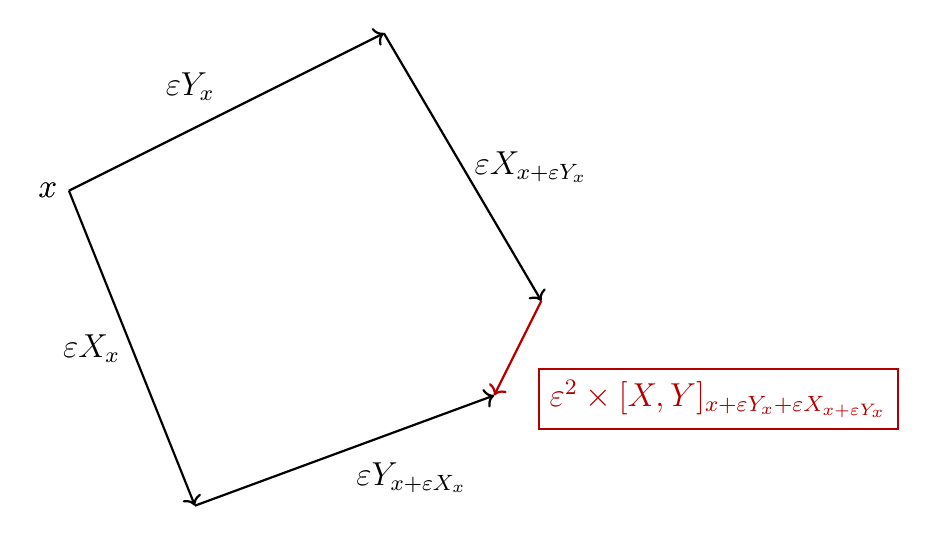
\begin{tikzpicture}[scale=2]
\draw[thick, ->] (0,0) node[left]{$x$} -- (2,1) node[midway, above left]{$\varepsilon Y_x$};
\draw[thick, ->] (2,1) --++ (1, -1.7) coordinate (A) {} node[midway, right] {$\varepsilon X_{x+ \varepsilon Y_x}$};
\draw[thick, ->] (0,0) node[left]{$x$} -- (0.8,-2) node[midway, left]{$\varepsilon X_x$};
\draw[thick, ->] (0.8,-2) --++ (1.9,0.7) node[midway, below right] {$\varepsilon Y_{x+ \varepsilon X_x}$};
\draw[thick, <-, red!70!black] (0.8,-2) ++ (1.9,0.7) -- (A) node[midway, below right=0.1in, rectangle, draw]{$\varepsilon^2 \times [X,Y]_{x + \varepsilon Y_x + \varepsilon X_{x + \varepsilon Y_x}}$};
\end{tikzpicture}
\caption{The definition of $[X,Y]$.}\label{fig:1}
\end{figure}

\begin{figure}[H]
\centering
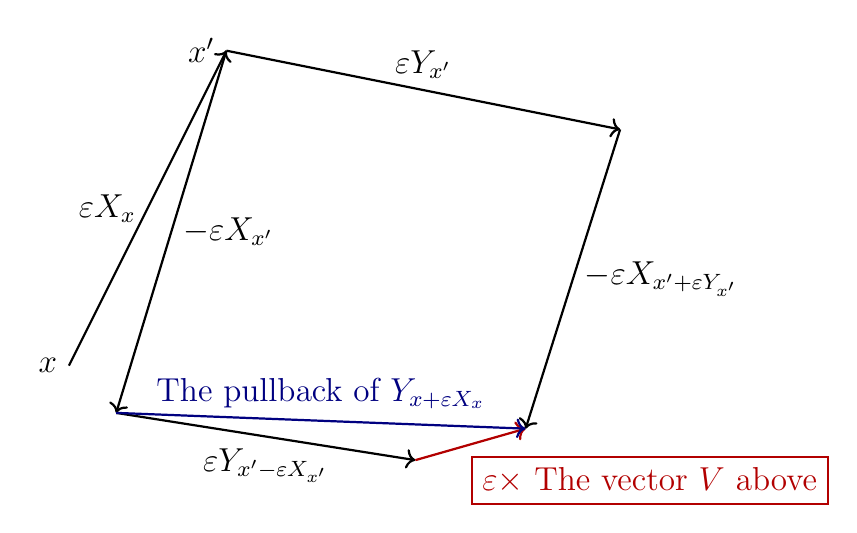
\begin{tikzpicture}[scale=2, every path/.style={thick,->}]
\coordinate (X) at (0,0) node[left] {$x$};
\path (X)++(1,2) coordinate (XX) node[left] {$x'$};
\path (XX)++(2.5,-0.5) coordinate (A) ++ (-0.6,-1.9) coordinate (B);
\path (XX) ++ (-0.7,-2.3) coordinate (C) ++(1.9,-0.3) coordinate (D);
\draw (X) -- (XX) node[left, midway] {$\varepsilon X_x$};
\draw (XX) -- (A) node[above, midway] {$\varepsilon Y_{x'}$};
\draw (A) -- (B) node[right, midway] {$- \varepsilon X_{x' + \varepsilon Y_{x'}}$};% node[right]{$x' + \varepsilon Y_{x'} - \varepsilon X_{x' + \varepsilon Y_{x'}}$};
\draw (XX) -- (C) node[right, midway] {$-\varepsilon X_{x'}$};
\draw (C) -- (D) node[below, midway] {$\varepsilon Y_{x' - \varepsilon X_{x'}}$};
\draw[red!70!black] (D) -- (B) node[below = 0.18in, right, midway, draw, rectangle] {$\varepsilon \times$ The vector $V$ above};
\draw[blue!50!black] (C) -- (B) node[midway, above] {The pullback of $Y_{x + \varepsilon X_x}$};
\end{tikzpicture}
\caption{The definition of $\Lie_X Y$.}\label{fig:2}
\end{figure}

Hopefully, from figure \ref{fig:2} it should become clear how this vector $V$ corresponds to the pullback of $Y_{x+\varepsilon X_x}$ minus $Y$. There's some basepoint trickery (maybe there's some clever way around it?), but I hope you'll believe me when I claim that $V$ corresponds to the difference between the pullback of $Y$ and $Y$ itself. Anyhow, to obtain the Lie derivative, we divide $V$ by $\varepsilon$, and so we get
\begin{equation}
V = \varepsilon (\Lie_X Y)_x... \text{ Ish.}
\end{equation}

We actually want $(\Lie_X Y)_x$ to be a vector tangent at $x$, so in truth $V / \varepsilon$ is actually $(\Lie_X Y)$ evaluated at some point with an ugly expression, which we call $x''$ because it comes up in the next paragraph. But this is where the digression with the product rule above comes in: \emph{Since $V$ is $(\Lie_X Y)$ evaluated at a point infinitesimally close to $X$, it is equal to $(\Lie_X Y)_x$ for practical purposes} (that is, up to infinitesimals).

Now, here is (finally) the punchline: comparing figures \ref{fig:1} and \ref{fig:2}, you should realize that \emph{$\varepsilon V$ is actually equal to $- \varepsilon^2 [-X,Y]_{x''}$}. (Beware the sign of $X$! This caused me a bit of a headache.) As such, $V/\varepsilon = [X,Y]_{x''}$, and hence $(\Lie_X Y)_{x''} = [X,Y]_{x''}$. This makes the connection between the Lie derivative and the Lie bracket as defined above. So now it remains to show that the Lie bracket defined as `infinitesimal noncommutativity' coincides with the usual definition $[X,Y] f = XY f - YX f$.

\section{Lie Bracket}

To discuss the usual definition of Lie bracket, we must discuss how a vector acts on a function by derivation.

We are seeing a vector as a pair of infinitesimally close points $x$ and $x + \varepsilon v$. Thus, the natural way to define the action of $v$ on a function $f$ would be as the number
\begin{equation}
v \cdot f = \frac{f(x + \varepsilon v) - f(x)}\varepsilon.
\end{equation}

As such, the expression $(Yf)_x$ should be taken to mean
\begin{equation}
(Yf)_x = \frac{f(x + \varepsilon Y_x) - f(x)}\varepsilon.
\end{equation}

Therefore, the term $(XYf)_x$ that appears in the usual bracket is written in long form as
\begin{equation}
\begin{aligned}
(XYf)_x &= \frac{(Yf)_{x + \varepsilon X_x} - (Yf)_x}\varepsilon\\
&=\frac{\frac{f(x + \varepsilon X_x + \varepsilon Y_{x + \varepsilon X_x}) - f(x + \varepsilon X_x)}\varepsilon - \frac{f(x + \varepsilon Y_x) - f(x)}\varepsilon}\varepsilon\\
&=\frac{f(x + \varepsilon X_x + \varepsilon Y_{x + \varepsilon X_x}) - f(x + \varepsilon X_x) - f(x + \varepsilon Y_x) + f(x)}{\varepsilon^2}.
\end{aligned}
\end{equation}

Now, writing $(XYf)_x - (YX f)_x$, it is clear that most terms cross out, and we obtain only
\begin{equation}\label{eq:b2}
(XYf)_x - (YX f)_x =\frac{f(x + \varepsilon X_x + \varepsilon Y_{x + \varepsilon X_x}) - f(x + \varepsilon Y_x + \varepsilon X_{x + \varepsilon Y_x})}{\varepsilon^2}.
\end{equation}

The right-hand side looks weird, but it can be tamed as follows. Set $x' = x + \varepsilon Y_x + \varepsilon X_{x + \varepsilon Y_x}$, which is the expression the rightmost $f$ is evaluated on. Then, going all the way to equation \eqref{eq:bracket} and figure \ref{fig:1}, we see that the leftmost $f$ is evaluated on
\begin{equation}
x + \varepsilon X_x + \varepsilon Y_{x + \varepsilon X_x} = x' + \varepsilon^2 [X,Y]_{x'}.
\end{equation}

Thus, from equation \eqref{eq:b2} we get
\begin{equation}
(XYf)_x - (YX f)_x =\frac{f(x' + \varepsilon^2 [X,Y]_{x'}) - f(x')}{\varepsilon^2}.
\end{equation}

Now, this expression doesn't look like a derivative, because we have a $\varepsilon^2$; it looks more like a second derivative. But realize that $\varepsilon^2$ is an infinitesimal, smaller than $\varepsilon$ itself, but an infinitesimal nonetheless. If we rename it to $\delta$, we see that
\begin{equation}
(XYf)_x - (YX f)_x =\frac{f(x' + \delta [X,Y]_{x'}) - f(x')}{\delta},
\end{equation}
which is clearly the same, \emph{by definition}, as $([X,Y] \cdot f)_{x'}$. Now we have again the detail of point of evaluation, and again, since $x'$ is infinitesimally close to $x$ itself, these coincide for practical intents and purposes, hence
\begin{equation}
[X,Y] \cdot f = XYf - YXf.
\end{equation}

This shows that the usual notion of Lie bracket coincides with the notion of `infinitesimal noncommutativity of sum', which ties everything together and shows that the Lie bracket coincides with the Lie derivative.
\end{document}